\documentclass[conference]{IEEEtran}
\usepackage[utf8]{inputenc}
\usepackage[spanish]{babel}
\usepackage{graphicx}
\usepackage{xurl}
\usepackage{cite}
\usepackage{booktabs}
\usepackage{array}
\usepackage{tabularx}
\usepackage{placeins}

\newcommand{\placeholderfigure}[2]{%
\begin{center}
\fbox{\begin{minipage}[c][#1][c]{0.94\linewidth}
\centering #2
\end{minipage}}
\end{center}
}

\begin{document}

\title{Deep Shadows}

\author{
\IEEEauthorblockN{Cristian Fuentes, Geremy Jurado, Manuel Polo, Andrés Barandica, Andrés Issa e Issac Gonzalez}
\IEEEauthorblockA{\textit{Pineapple Engine} \\
Universidad del Norte \\
Barranquilla, Colombia}
}

\maketitle

\begin{abstract}
Este artículo presenta el diseño y desarrollo de \textit{Deep Shadows}, un videojuego 2D de plataformas creado por Pineapple Engine para generar conciencia sobre las consecuencias emocionales del bullying. El proyecto abordó el problema mediante una experiencia interactiva en la que el jugador controla a un protagonista que atraviesa espacios escolares y simbólicos marcados por pensamientos intrusivos, distorsión visual y obstáculos asociados al acoso. La solución fue implementada en Godot con GDScript y se estructuró con fundamentos de programación orientada a objetos, incluyendo clases propias para jugador, enemigos, puzzles, guardado, habilidades, interfaz, diálogos y control de niveles. La metodología integró requisitos funcionales, requisitos no funcionales basados en FURPS, uso de patrones de diseño y una prueba de usabilidad con usuarios externos. Como resultado, se obtuvo un prototipo jugable con menú, slots de partida, opciones de accesibilidad, manual de controles, movimiento, salto, sprint con estamina, puzzles aleatorios, gafas temporales, HUD, enemigos, checkpoints, diálogos y progresión entre mundos. Se concluye que el videojuego permite comunicar el impacto del bullying desde mecánicas comprensibles y una arquitectura técnica defendible.
\end{abstract}

\begin{abstract}
This paper presents the design and development of \textit{Deep Shadows}, a 2D platform video game created by Pineapple Engine to raise awareness about the emotional consequences of bullying. The project approached the problem through an interactive experience in which the player controls a protagonist who moves through school and symbolic spaces shaped by intrusive thoughts, visual distortion, and obstacles related to harassment. The solution was implemented in Godot using GDScript and structured under object-oriented programming principles, including custom classes for the player, enemies, puzzles, save system, abilities, interface, dialogues, and level control. The methodology integrated functional requirements, non-functional requirements based on FURPS, design patterns, and usability testing with external users. As a result, a playable prototype was obtained with a menu, save slots, accessibility options, controls manual, movement, jumping, stamina-based sprinting, random puzzles, temporary glasses activation, HUD, enemies, checkpoints, dialogues, and world progression. The project concludes that the game can communicate the impact of bullying through understandable gameplay mechanics and a technically defensible software architecture.
\end{abstract}

\begin{IEEEkeywords}
Bullying, videojuegos serios, Godot, GDScript, Programación Orientada a Objetos, usabilidad, accesibilidad.
\end{IEEEkeywords}

\section{Introducción}
El bullying es una forma de acoso intencionado y repetido que ocurre cuando una persona o grupo ejerce una relación de poder desfavorable sobre otra. Esta problemática no solo produce afectaciones inmediatas en la convivencia escolar, sino que también puede dejar secuelas emocionales que se mantienen en el tiempo, como ansiedad, inseguridad, aislamiento, miedo al rechazo y dificultad para relacionarse con otros. En el caso del ciberacoso, estas consecuencias pueden intensificarse porque la agresión se expande a espacios digitales, permanece visible y puede ser observada por múltiples espectadores.

Aunque muchas intervenciones contra el bullying se apoyan en charlas, campañas o materiales informativos, los videojuegos serios permiten representar situaciones sociales complejas mediante acciones, decisiones, retroalimentación y consecuencias. De esta manera, el jugador no solo recibe información, sino que participa en un entorno simulado donde las reglas del juego pueden simbolizar emociones, obstáculos internos y procesos de superación. Esta característica es relevante para una población joven, familiarizada con experiencias interactivas y con dinámicas de aprendizaje visual.

\textit{Deep Shadows} propone un videojuego 2D de plataformas orientado a jóvenes y adolescentes. El protagonista atraviesa escenarios oscuros en los que la visión se distorsiona, aparecen pensamientos negativos y se deben resolver retos para avanzar. La mecánica de las gafas representa la búsqueda de claridad: al activarlas, el jugador puede ver mejor el entorno, acceder a elementos ocultos y enfrentar retos asociados a la presión social. El objetivo general del proyecto es implementar un videojuego funcional relacionado con el bullying que use fundamentos de programación orientada a objetos y que comunique una reflexión sobre las consecuencias emocionales del acoso.

\section{Contribuciones}
Las principales contribuciones del proyecto son las siguientes:

\begin{itemize}
    \item Se diseñó una propuesta lúdica original sobre bullying que evita el formato de preguntas explícitas sobre el tema y usa mecánicas, escenarios y diálogos como metáforas jugables.
    \item Se implementó un prototipo funcional en Godot con menú principal, sistema de partidas, opciones, manual de usuario, mundos, HUD, puzzles aleatorios, enemigos y progresión.
    \item Se aplicaron fundamentos de programación orientada a objetos mediante clases propias, herencia, encapsulamiento, composición, señales y polimorfismo.
    \item Se incorporaron patrones de diseño defendibles: \textit{State} para los estados del jugador y \textit{Observer} mediante señales de Godot para desacoplar eventos del juego.
    \item Se incluyeron elementos de accesibilidad y usabilidad, como filtros de color para daltonismo, control de volumen, resolución, modo de pantalla, intensidad de sacudida de cámara y una escena de controles.
\end{itemize}

\section{Trabajos Relacionados}
Los videojuegos serios han sido estudiados como herramientas de prevención, sensibilización y evaluación en situaciones de bullying y ciberacoso. Calvo-Morata et al. desarrollaron y validaron \textit{Conectado}, un videojuego serio para aumentar la conciencia sobre bullying y cyberbullying en jóvenes. El estudio combinó cuestionarios y analíticas de juego, y reportó un efecto positivo en el aumento de conciencia de los participantes \cite{calvo2021}.

Ferreira et al. analizaron el juego serio \textit{Com@Viver} con estudiantes de séptimo y octavo grado. Su objetivo fue estudiar si una experiencia multijugador podía fomentar empatía cognitiva y afectiva en observadores de ciberacoso. Los resultados cuantitativos y cualitativos indicaron mayores niveles de empatía y prosocialidad en quienes jugaron \cite{ferreira2021}. Este antecedente es importante para \textit{Deep Shadows}, porque evidencia que una experiencia interactiva puede provocar reflexión sobre roles sociales y consecuencias emocionales.

Francisco et al. estudiaron actividades gamificadas asociadas a un juego serio sobre cyberbullying, enfocándose en la relación entre empatía y desconexión moral. Sus resultados mostraron que participantes con mayor empatía presentaron menores niveles de desconexión moral durante el tiempo de intervención \cite{francisco2024}. Esta investigación respalda la inclusión de mensajes y situaciones que invitan a reconocer el daño causado por el acoso.

Martel-Santana y Martín-del-Pozo evaluaron la usabilidad de \textit{About Us}, un juego serio tipo RPG para tratar bullying y cyberbullying en educación primaria. El estudio encontró una valoración positiva por parte de 98 docentes en formación, lo que resalta la importancia de evaluar no solo el contenido, sino también la facilidad de uso del recurso \cite{martel2025}.

Brečko et al. evaluaron el \textit{CyberSafe Tool}, una intervención educativa basada en juego serio sobre cyberviolencia. La intervención fue aplicada a 959 adolescentes entre 13 y 16 años y usó mediciones antes, inmediatamente después y tres semanas después. Los resultados indicaron cambios positivos de actitud que se mantuvieron en la medición posterior \cite{brecko2024}. Este trabajo confirma la utilidad de integrar narrativa, roles y discusión guiada para abordar problemáticas sociales.

Finalmente, el CONICET reportó iniciativas recientes de videojuegos y simulaciones virtuales para prevenir grooming y bullying en infancia y adolescencia, destacando el potencial de los \textit{serious games} para educar, sensibilizar y transformar conductas desde edades tempranas \cite{conicet2025}. Estos antecedentes muestran que \textit{Deep Shadows} se ubica dentro de una línea actual de soluciones interactivas que buscan generar conciencia social mediante experiencias jugables.

\section{Metodología}
\subsection{Empresa, Roles y Gestión}
El grupo de trabajo se identificó como Pineapple Engine. La asignación de roles quedó distribuida de la siguiente manera: Cristian Fuentes como gerente de proyectos, Andrés Issa como director de diseño, Geremy Jurado como director de pruebas, Manuel Polo como director de documentación, Andrés Barandica como director de UI/UX e Issac Gonzalez como director de UI/UX. Aunque el lineamiento general contempla grupos de tres a cinco integrantes, el equipo contó con un sexto miembro por una situación especial de reasignación aprobada durante el desarrollo del curso. Esta distribución permitió separar responsabilidades de coordinación, diseño de la solución, pruebas, documentación e interfaz de usuario.

Para la gestión de actividades se utilizó Trello como herramienta de seguimiento del proyecto. El tablero del equipo se encuentra disponible en \url{https://trello.com/b/wAE43TkV/poo}. En este espacio se organizaron las tareas por áreas de trabajo, se registró el avance del desarrollo y se evidenció la asignación de responsabilidades por rol. \textbf{[COMPLETAR: agregar una captura del tablero o describir brevemente las listas usadas, por ejemplo: pendientes, en proceso, pruebas y terminado.]}

\subsection{Enfoque del Juego}
La propuesta seleccionada fue un videojuego de plataformas 2D con ambientación de fantasía, suspenso y espacios escolares. El jugador controla a un protagonista que debe avanzar por escenarios oscuros, superar obstáculos, resolver puzzles y enfrentar enemigos. La problemática del bullying se expresa mediante distorsión visual, pensamientos negativos, puertas bloqueadas, retos de memoria y situaciones asociadas al salón o al pasillo.

La población objetivo corresponde a jóvenes y adolescentes con experiencia básica en videojuegos de teclado. La decisión de usar un juego de plataformas se justificó porque este género permite combinar habilidad motriz, exploración, obstáculos, recompensas y progresión narrativa sin depender de preguntas directas sobre bullying. Esto cumple el lineamiento de evitar juegos tipo cuestionario.

\subsection{Metodología de Desarrollo}
El desarrollo se organizó con una metodología incremental. En una primera etapa se definieron el concepto del juego, la problemática, los requisitos y el diseño de clases. Luego se implementó un corte vertical del prototipo con movimiento, salto, sprint, HUD, puerta, llave y puzzle. En iteraciones posteriores se agregaron la habilidad de gafas, distorsión visual, sistema de guardado por slots, menú de opciones, escena de controles, enemigos, diálogos, checkpoints, puzzles temáticos, segundo mundo y mejoras de accesibilidad.

\subsection{Requerimientos Funcionales}
La Tabla \ref{tab:req-funcionales} resume los requerimientos funcionales definidos para el prototipo.

\begin{table*}[t]
\caption{Requerimientos funcionales del videojuego}
\label{tab:req-funcionales}
\centering
\begin{tabularx}{\textwidth}{>{\raggedright\arraybackslash}p{1.2cm}X>{\raggedright\arraybackslash}p{3.6cm}}
\toprule
\textbf{ID} & \textbf{Descripción} & \textbf{Evidencia en el prototipo} \\
\midrule
RF-01 & El sistema debe permitir iniciar, cargar o eliminar una partida desde slots de guardado. & Menú de partidas y clase \textit{SistemaGuardado}. \\
RF-02 & El jugador debe desplazarse horizontalmente usando A/D o flechas direccionales. & Acciones \textit{mover\_izquierda} y \textit{mover\_derecha}. \\
RF-03 & El jugador debe saltar con la barra espaciadora. & Acción \textit{saltar} y método \textit{saltar()} en \textit{Jugador}. \\
RF-04 & El jugador debe ejecutar sprint con Shift y consumo de estamina. & Acción \textit{sprint}, \textit{SistemaEstamina} y \textit{EstadoJugadorSprint}. \\
RF-05 & El jugador debe interactuar con objetos usando la tecla E. & Acción \textit{interactuar}, llave, puerta, altar, tótems y NPC. \\
RF-06 & El jugador debe activar gafas con Q durante un tiempo limitado. & \textit{HabilidadGafas}, HUD de gafas y distorsión visual. \\
RF-07 & El juego debe incluir puzzles con componentes aleatorios. & \textit{PuzzleMatematicas}, \textit{PuzzleSecuencia} y \textit{PuzzleGafas}. \\
RF-08 & El juego debe mostrar mensajes de ayuda durante la partida. & HUD, diálogos, mensajes automáticos y escena de controles. \\
RF-09 & El jugador debe enfrentar obstáculos, enemigos o amenazas con comportamientos diferentes. & Enemigos de patrulla, persecución, flotantes, jefe y muro. \\
RF-10 & El sistema debe permitir pausar, reiniciar y volver al menú. & \textit{MenuPausa} y acciones de pausa/reinicio. \\
RF-11 & El usuario debe poder modificar opciones de audio, pantalla y accesibilidad. & Menú de opciones con volumen, resolución, modo de pantalla, filtros de color y sacudida de cámara. \\
\bottomrule
\end{tabularx}
\end{table*}

\subsection{Requerimientos No Funcionales}
Los requisitos no funcionales se organizaron usando el modelo FURPS, que clasifica atributos de calidad en funcionalidad, usabilidad, confiabilidad, rendimiento y soporte \cite{grady1992}. La Tabla \ref{tab:furps} presenta la aplicación del modelo al proyecto.

\begin{table*}[t]
\caption{Requerimientos no funcionales basados en FURPS}
\label{tab:furps}
\centering
\begin{tabularx}{\textwidth}{>{\raggedright\arraybackslash}p{2.4cm}X}
\toprule
\textbf{Categoría} & \textbf{Requisito} \\
\midrule
Funcionalidad & El juego debe integrar mecánicas coherentes con el objetivo de concientización: obstáculos, pensamientos narrativos, visión distorsionada, gafas, puzzles, diálogos y progresión entre mundos. \\
Usabilidad & El usuario debe entender controles y objetivos mediante menú principal, manual de usuario, HUD, mensajes dentro del juego, menú de pausa y retroalimentación visual. Se realizará una prueba con al menos cinco usuarios. \\
Confiabilidad & El juego debe continuar funcionando ante entradas inesperadas, repetición de botones, cancelación de puzzles, caídas del mapa, reinicios y carga de partidas guardadas. \\
Rendimiento & El prototipo debe ejecutarse de forma fluida en un computador de laboratorio o equipo promedio, manteniendo una respuesta inmediata a los controles. \textbf{[COMPLETAR: equipo usado y FPS aproximado si lo midieron.]}
\\
Soporte & El código debe estar dividido en clases y escenas mantenibles, con nombres claros, señales y responsabilidades separadas para facilitar cambios futuros. \\
\bottomrule
\end{tabularx}
\end{table*}

\subsection{Componente Inclusivo}
Aunque inicialmente se consideró una selección de \textit{skin}, en la versión actual el componente inclusivo se orientó hacia accesibilidad visual y comodidad de interacción. El menú de opciones permite seleccionar filtros de color para distintos tipos de daltonismo, modificar el volumen, probar sonido, ajustar resolución, cambiar modo de pantalla y regular la sacudida de cámara. Adicionalmente, el juego presenta instrucciones visuales mediante el manual de usuario, mensajes dentro del HUD y textos de retroalimentación en puzzles.

\subsection{Arquitectura Orientada a Objetos}
El diseño del juego se basó en clases propias de GDScript. Godot permite registrar scripts como clases mediante \textit{class\_name}, usar herencia con \textit{extends}, definir señales y organizar la lógica en nodos y escenas \cite{godotdocs}. En el prototipo se identificaron más de cinco clases de autoría propia, por lo que se cumple el mínimo exigido en la consigna.

\begin{itemize}
    \item \textbf{Jugador}: administra vida, movimiento, salto, sprint, daño, invulnerabilidad, animaciones y gafas.
    \item \textbf{SistemaEstamina}: encapsula el consumo, regeneración y porcentaje de estamina.
    \item \textbf{HabilidadGafas}: controla duración, enfriamiento, activación y señales de estado de las gafas.
    \item \textbf{SistemaGuardado}: administra slots, carga, guardado, borrado de partidas y transición entre escenas.
    \item \textbf{EstadoJugadorBase}: define la interfaz común para estados del jugador.
    \item \textbf{EstadoJugadorNormal, EstadoJugadorSprint, EstadoJugadorBloqueado y EstadoJugadorAturdido}: implementan el patrón \textit{State}.
    \item \textbf{EnemigoBase}: define vida, daño, movimiento base y ataque por contacto.
    \item \textbf{EnemigoPatrulla, EnemigoPerseguidor y EnemigoFlotanteBase}: especializan comportamientos enemigos mediante herencia.
    \item \textbf{PuzzleBase, PuzzleMatematicas, PuzzleSecuencia y PuzzleGafas}: modelan retos interactivos, cancelación, completado y generación aleatoria.
    \item \textbf{HUD}: presenta vida, estamina, gafas, llave, checkpoints, mensajes y pensamientos.
    \item \textbf{MainGame y Mundo2}: coordinan configuración de niveles, puertas, checkpoints, enemigos, puzzles, pausas y progresión.
    \item \textbf{DialogoUI y NPCDialogo}: administran interacción narrativa con personajes y mensajes.
\end{itemize}

\begin{figure*}[t]
\centering
\IfFileExists{figuras/uml_clases_final.png}{%
\includegraphics[width=0.95\textwidth]{figuras/uml_clases_final.png}
}{%
\placeholderfigure{5cm}{Insertar aquí el UML de clases final exportado como figuras/uml\_clases\_final.png. Debe incluir como mínimo: MainGame, Mundo2, Jugador, SistemaEstamina, HabilidadGafas, SistemaGuardado, estados del jugador, EnemigoBase, enemigos concretos, PuzzleBase, PuzzleMatematicas, PuzzleSecuencia, PuzzleGafas, HUD y DialogoUI.}
}
\caption{Diagrama de clases propuesto para \textit{Deep Shadows}.}
\label{fig:diagrama-clases}
\end{figure*}

\subsection{Patrones de Diseño}
El patrón \textit{State} se usó para separar el comportamiento del jugador en estados como normal, sprint, bloqueado y aturdido. Esto evita concentrar toda la lógica de movimiento en una sola clase con múltiples condicionales, y facilita agregar nuevos estados sin modificar de forma agresiva la clase \textit{Jugador}.

El patrón \textit{Observer} se implementó mediante señales de Godot. La documentación de Godot describe las señales como su versión del patrón observador y permite conectarlas desde el editor o por código \cite{godotsignals}. En el prototipo, el jugador emite señales cuando cambia la vida, la estamina, el sprint o el estado de las gafas; el HUD escucha esas señales y actualiza la interfaz sin consultar constantemente el estado interno del jugador.

\subsection{Lenguaje y Plataforma}
La plataforma escogida fue Godot, usando GDScript como lenguaje principal. Esta decisión se justificó por tres razones. Primero, Godot ofrece soporte nativo para juegos 2D mediante escenas, nodos, colisiones, cámaras, señales y manejo de entrada. Segundo, GDScript se integra directamente con el editor y permite crear clases propias de manera clara. Tercero, el motor facilita exportar y ejecutar prototipos sin depender de licencias comerciales.

El mapa de entradas de Godot permitió definir acciones como movimiento, salto, sprint, interacción, uso de gafas, pausa y reinicio. La documentación oficial recomienda configurar acciones en el \textit{Input Map} y consultar esas acciones desde código, lo cual favorece que los controles puedan cambiarse sin modificar toda la lógica del jugador \cite{godotinput}.

\subsection{Uso de Inteligencia Artificial}
Durante la preparación del informe se utilizó Codex como apoyo para revisar la consigna, contrastar requisitos con el código existente, organizar la estructura del artículo y proponer redacción técnica. La herramienta no reemplazó la validación del grupo ni la ejecución del software; su uso se limitó a asistencia en documentación, análisis del repositorio y mejora de claridad del informe.

\section{Resultados}
\subsection{Estado del Prototipo}
El prototipo actual incluye un menú principal, menú de opciones, manual de usuario, selector de partidas con tres slots, escena de juego principal, HUD, jugador, puzzles, puertas, llave, checkpoints, enemigos, sistema de diálogos, segundo mundo y elementos de accesibilidad. La Tabla \ref{tab:resultados-poo} resume evidencias de programación orientada a objetos observadas en el proyecto.

\begin{table*}[t]
\caption{Evidencias de programación orientada a objetos}
\label{tab:resultados-poo}
\centering
\begin{tabularx}{\textwidth}{>{\raggedright\arraybackslash}p{2.8cm}X}
\toprule
\textbf{Fundamento} & \textbf{Evidencia en el código} \\
\midrule
Clases propias & Scripts con \textit{class\_name}: \textit{Jugador}, \textit{SistemaEstamina}, \textit{HabilidadGafas}, \textit{SistemaGuardado}, \textit{HUD}, \textit{MainGame}, \textit{Mundo2}, \textit{PuzzleBase}, \textit{PuzzleMatematicas}, \textit{EnemigoBase}, entre otros. \\
Encapsulamiento & La estamina, las gafas y el guardado se administran desde clases separadas con métodos de consumo, regeneración, activación, consulta, carga y escritura. \\
Herencia & \textit{EnemigoPatrulla}, \textit{EnemigoPerseguidor}, \textit{EnemigoFlotanteBase} y \textit{JefeSombras} derivan de \textit{EnemigoBase}; los puzzles concretos derivan de \textit{PuzzleBase}. \\
Polimorfismo & Los enemigos y puzzles sobrescriben métodos de comportamiento para moverse, perseguir, patrullar, flotar o generar retos distintos. \\
Composición & \textit{Jugador} contiene instancias de \textit{SistemaEstamina}, \textit{HabilidadGafas} y estados del jugador. \\
Patrones & Se evidencian \textit{State} en los estados del jugador y \textit{Observer} mediante señales entre jugador, HUD, enemigos y controlador principal. \\
\bottomrule
\end{tabularx}
\end{table*}

\FloatBarrier

\subsection{Evidencias Visuales}
Las Figuras \ref{fig:menu} a \ref{fig:puzzle-eco} muestran evidencias visuales del prototipo, incluyendo menús, controles, sistema de partidas, escenario inicial y puzzles.

\begin{figure}[!htbp]
\centering
\IfFileExists{figuras/menu_principal.png}{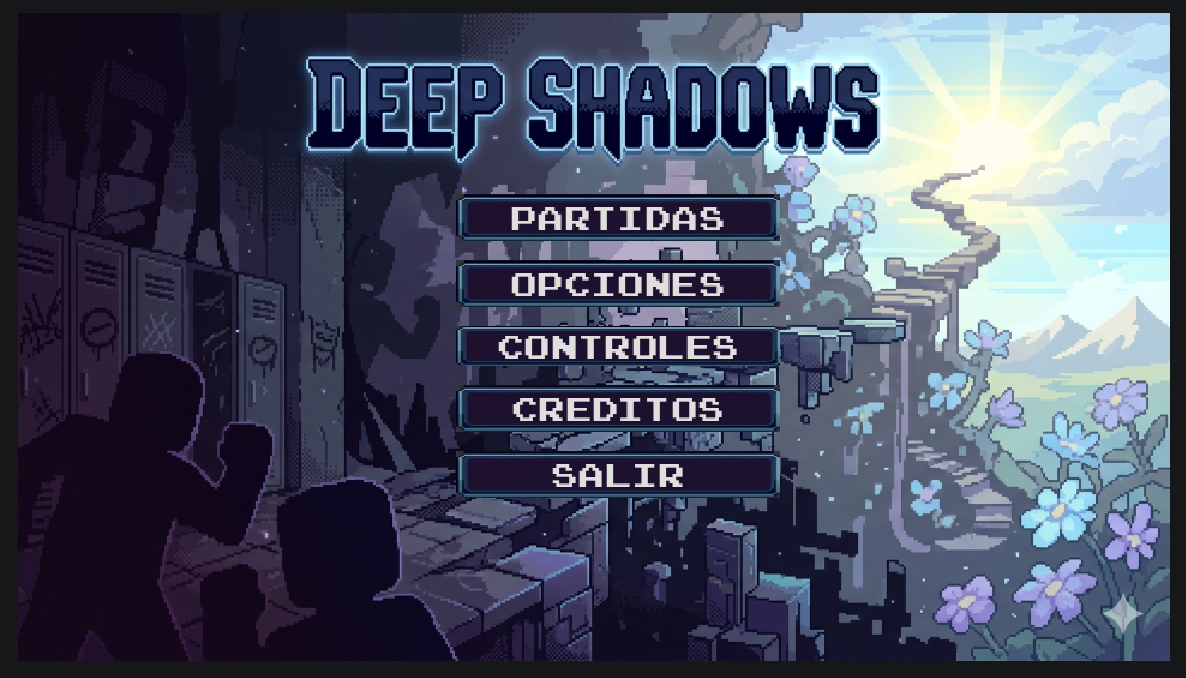
\includegraphics[width=\linewidth]{figuras/menu_principal.png}}{\placeholderfigure{3.1cm}{Guardar captura como figuras/menu\_principal.png}}
\caption{Menú principal de \textit{Deep Shadows}.}
\label{fig:menu}
\end{figure}

\begin{figure}[!htbp]
\centering
\IfFileExists{figuras/opciones.png}{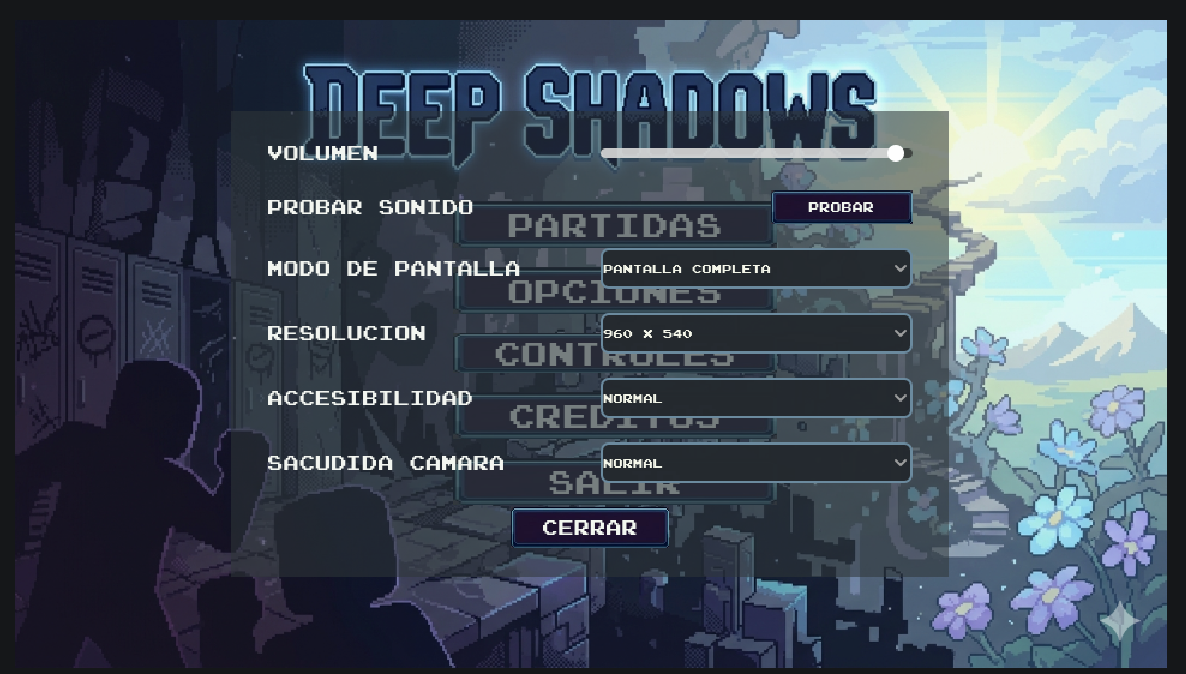
\includegraphics[width=\linewidth]{figuras/opciones.png}}{\placeholderfigure{3.1cm}{Guardar captura como figuras/opciones.png}}
\caption{Menú de opciones con volumen, pantalla, resolución, accesibilidad y sacudida de cámara.}
\label{fig:opciones}
\end{figure}

\begin{figure}[!htbp]
\centering
\IfFileExists{figuras/controles.png}{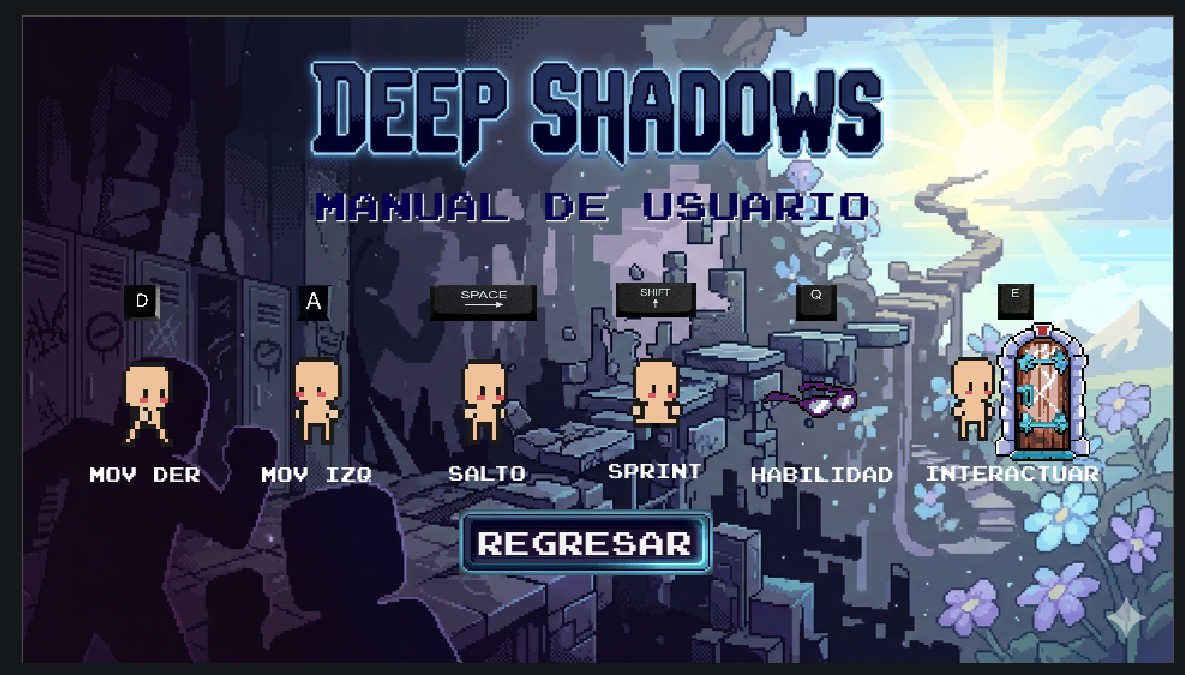
\includegraphics[width=\linewidth]{figuras/controles.png}}{\placeholderfigure{3.1cm}{Guardar captura como figuras/controles.png}}
\caption{Manual de usuario con controles principales del juego.}
\label{fig:controles}
\end{figure}

\begin{figure}[!htbp]
\centering
\IfFileExists{figuras/slots_partidas.png}{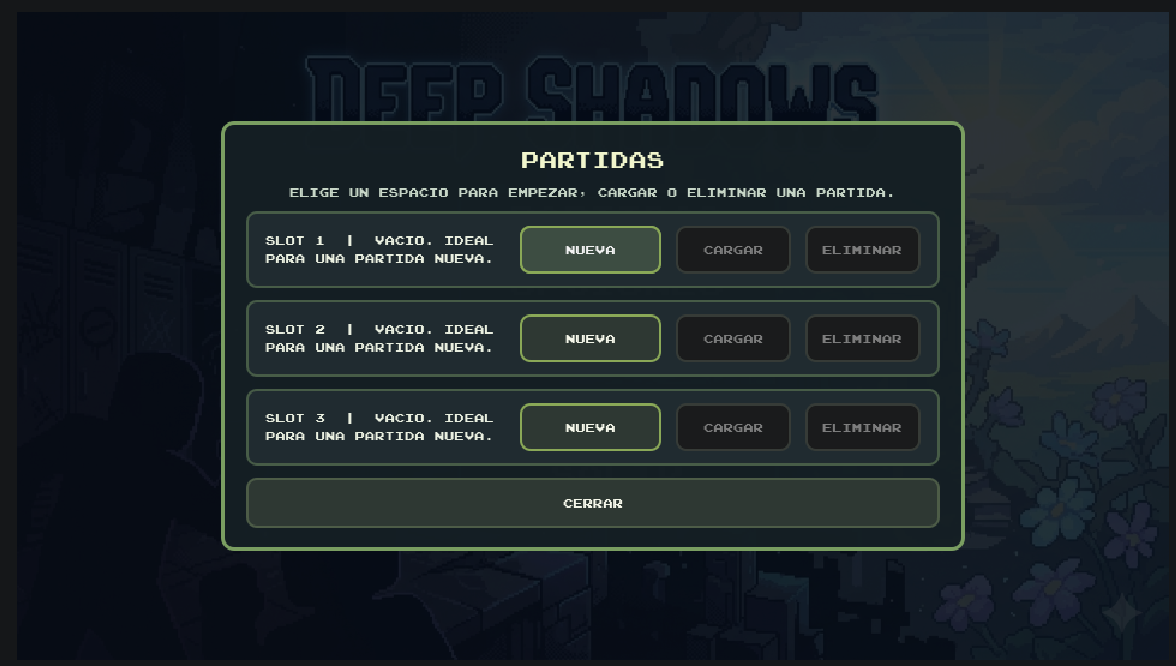
\includegraphics[width=\linewidth]{figuras/slots_partidas.png}}{\placeholderfigure{3.1cm}{Guardar captura como figuras/slots\_partidas.png}}
\caption{Selector de partidas con opciones para crear, cargar o eliminar guardados.}
\label{fig:slots}
\end{figure}

\begin{figure}[!htbp]
\centering
\IfFileExists{figuras/primer_escenario.png}{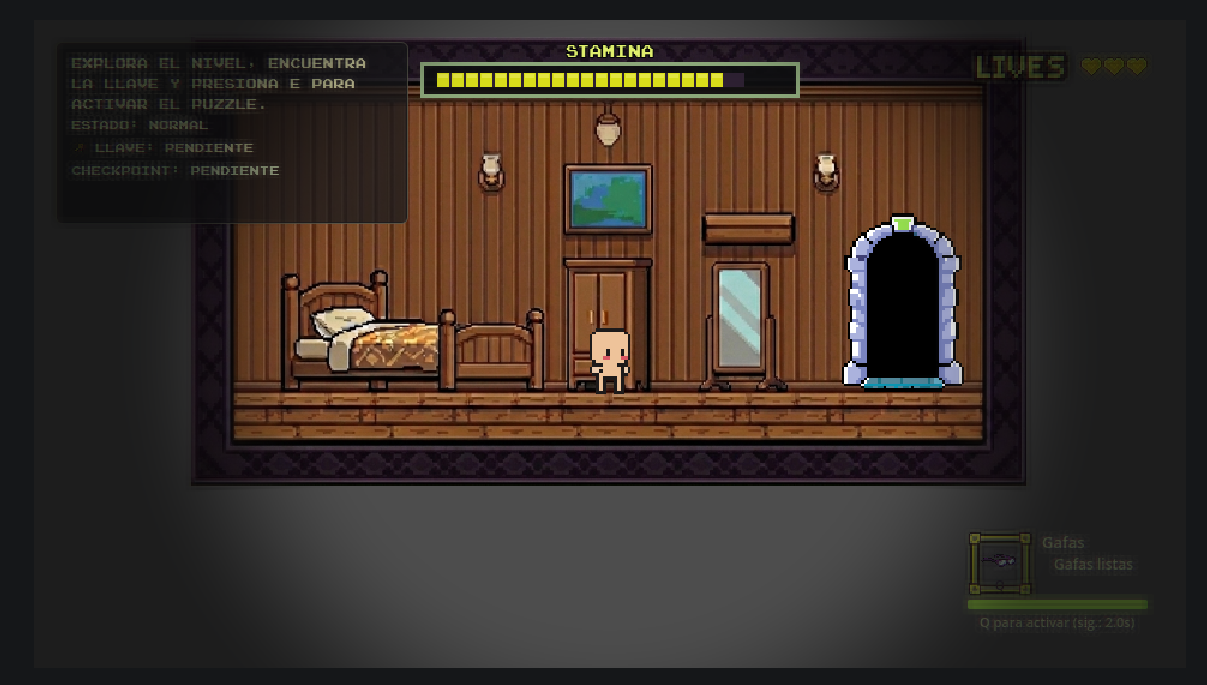
\includegraphics[width=\linewidth]{figuras/primer_escenario.png}}{\placeholderfigure{3.1cm}{Guardar captura como figuras/primer\_escenario.png}}
\caption{Primer escenario jugable con HUD, estamina, vidas y mensajes de orientación.}
\label{fig:escenario}
\end{figure}

\begin{figure}[!htbp]
\centering
\IfFileExists{figuras/puzzle_salon.png}{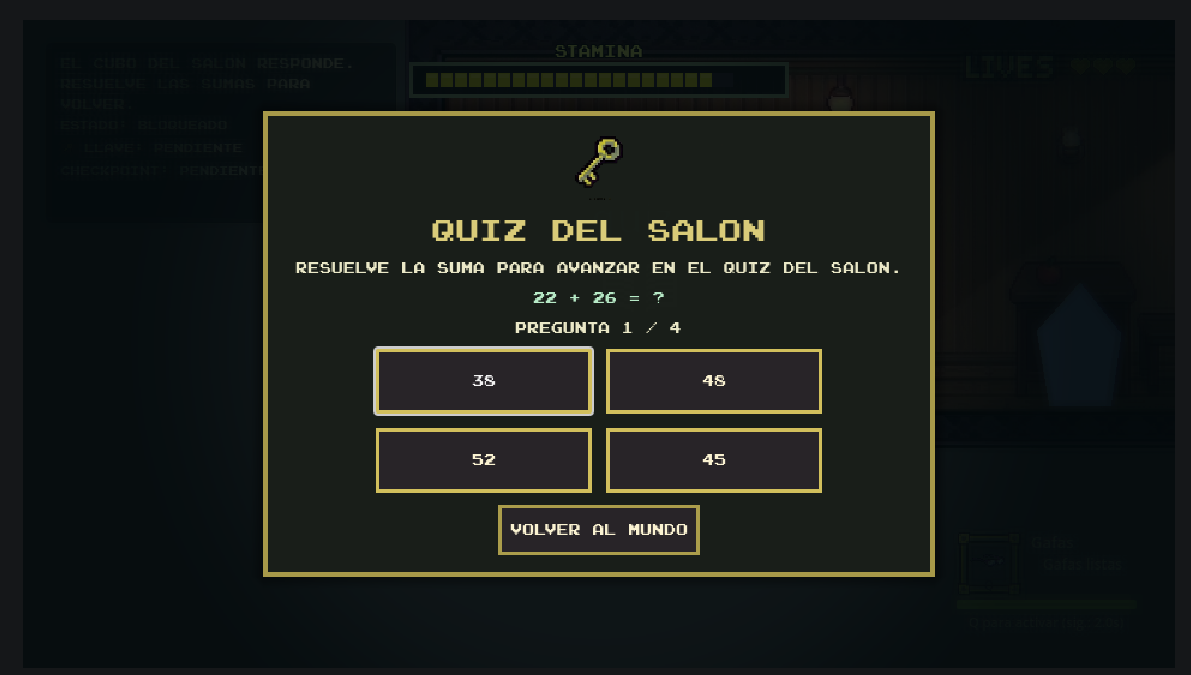
\includegraphics[width=\linewidth]{figuras/puzzle_salon.png}}{\placeholderfigure{3.1cm}{Guardar captura como figuras/puzzle\_salon.png}}
\caption{Primer puzzle: quiz del salón con sumas aleatorias.}
\label{fig:puzzle-salon}
\end{figure}

\begin{figure}[!htbp]
\centering
\IfFileExists{figuras/puzzle_eco.png}{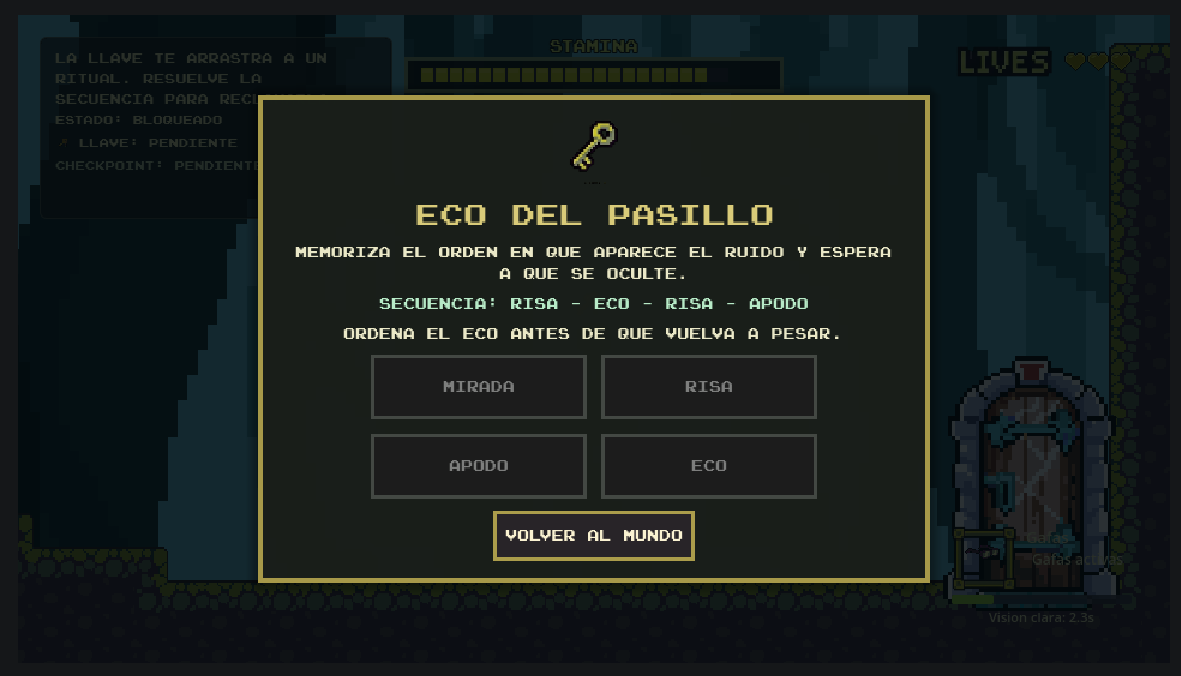
\includegraphics[width=\linewidth]{figuras/puzzle_eco.png}}{\placeholderfigure{3.1cm}{Guardar captura como figuras/puzzle\_eco.png}}
\caption{Segundo puzzle: eco del pasillo basado en memoria y secuencia.}
\label{fig:puzzle-eco}
\end{figure}

\FloatBarrier

\subsection{Prueba de Usabilidad}
La consigna exige realizar una prueba de usabilidad con al menos cinco usuarios. Para esta evaluación se propone un protocolo breve basado en pruebas con tareas representativas, como recomienda Nielsen Norman Group para estudios cualitativos con cinco usuarios \cite{nielsen2012}. Cada participante debe jugar el prototipo y completar las tareas de la Tabla \ref{tab:tareas-usabilidad}.

\begin{table}[!htbp]
\caption{Tareas propuestas para la prueba de usabilidad}
\label{tab:tareas-usabilidad}
\centering
\begin{tabularx}{\linewidth}{>{\raggedright\arraybackslash}p{0.9cm}X}
\toprule
\textbf{ID} & \textbf{Tarea} \\
\midrule
T1 & Iniciar una partida nueva desde un slot de guardado. \\
T2 & Consultar la pantalla de controles e identificar las teclas principales. \\
T3 & Moverse, saltar y usar sprint hasta superar una zona inicial. \\
T4 & Resolver el puzzle del salón. \\
T5 & Activar las gafas y resolver el puzzle del pasillo. \\
T6 & Modificar una opción de accesibilidad o pantalla y volver al menú. \\
\bottomrule
\end{tabularx}
\end{table}

Al finalizar, se debe aplicar una encuesta corta con escala de 1 a 5 para medir claridad de controles, comprensión del objetivo, dificultad, atractivo visual, utilidad de mensajes, estabilidad y percepción del tema tratado. La Tabla \ref{tab:resultados-usabilidad} queda preparada para completar con los resultados reales.

\begin{table}[!htbp]
\caption{Resultados de la prueba de usabilidad}
\label{tab:resultados-usabilidad}
\centering
\scriptsize
\begin{tabularx}{\linewidth}{>{\raggedright\arraybackslash}p{0.55cm}>{\raggedright\arraybackslash}p{1.15cm}>{\raggedright\arraybackslash}p{1.15cm}X}
\toprule
\textbf{Usuario} & \textbf{Tareas} & \textbf{Dificultad} & \textbf{Observaciones principales} \\
\midrule
U1 & \textbf{[ ]/6} & \textbf{[ ]/5} & \textbf{[COMPLETAR]} \\
U2 & \textbf{[ ]/6} & \textbf{[ ]/5} & \textbf{[COMPLETAR]} \\
U3 & \textbf{[ ]/6} & \textbf{[ ]/5} & \textbf{[COMPLETAR]} \\
U4 & \textbf{[ ]/6} & \textbf{[ ]/5} & \textbf{[COMPLETAR]} \\
U5 & \textbf{[ ]/6} & \textbf{[ ]/5} & \textbf{[COMPLETAR]} \\
\bottomrule
\end{tabularx}
\end{table}

\subsection{Análisis de Usabilidad}
\textbf{[COMPLETAR DESPUÉS DE LA PRUEBA]} A partir de los resultados, se debe reportar cuántos usuarios completaron cada tarea, qué errores fueron más frecuentes, qué mensajes no se entendieron, qué partes generaron mayor dificultad y qué ajustes se realizaron después de observar a los participantes. También se recomienda incluir una gráfica sencilla con el promedio de calificación por criterio.

\FloatBarrier

\section{Conclusiones}
\textit{Deep Shadows} permitió desarrollar una solución interactiva relacionada con el bullying mediante un videojuego 2D de plataformas. El prototipo cumplió con requisitos centrales de la consigna: creación propia, componente aleatorio, interfaz gráfica, más de cinco clases de autoría propia y uso de patrones de diseño. La mecánica de visión distorsionada y gafas permitió representar de forma simbólica la dificultad de percibir el entorno después de experiencias de acoso, mientras que los mensajes internos del protagonista reforzaron el componente narrativo.

Desde el punto de vista técnico, el uso de Godot y GDScript facilitó una arquitectura organizada por escenas y clases. La separación entre jugador, estamina, gafas, puzzles, guardado, enemigos, HUD y controladores de mundo permitió aplicar conceptos de programación orientada a objetos y mantener una estructura defendible para la sustentación. Como limitación, el prototipo todavía requiere completar evidencias finales, resultados de usabilidad, cronograma de trabajo y capturas de etapas avanzadas del juego.

Como trabajo futuro, se mejorará el balance de dificultad, se ampliarán los mundos, se incluirán más eventos narrativos relacionados con apoyo emocional y se pulirá la accesibilidad del juego para que más usuarios puedan interactuar con la experiencia de manera cómoda.

\FloatBarrier

\begingroup
\sloppy
\begin{thebibliography}{00}

\bibitem{calvo2021}
A. Calvo-Morata, C. Alonso-Fernández, M. Freire, I. Martínez-Ortiz, and B. Fernández-Manjón, ``Creating awareness on bullying and cyberbullying among young people: Validating the effectiveness and design of the serious game Conectado,'' \textit{Telematics and Informatics}, vol. 60, 2021, Art. no. 101568, doi: 10.1016/j.tele.2021.101568.

\bibitem{ferreira2021}
P. C. Ferreira, A. M. Veiga Simão, A. Paiva, C. Martinho, R. Prada, A. Ferreira, and F. Santos, ``Exploring empathy in cyberbullying with serious games,'' \textit{Computers \& Education}, vol. 166, 2021, Art. no. 104155, doi: 10.1016/j.compedu.2021.104155.

\bibitem{francisco2024}
S. M. Francisco, P. C. Ferreira, A. M. Veiga Simão, and N. S. Pereira, ``Moral disengagement and empathy in cyberbullying: how they are related in reflection activities about a serious game,'' \textit{BMC Psychology}, vol. 12, Art. no. 168, 2024, doi: 10.1186/s40359-024-01582-3.

\bibitem{martel2025}
A. Martel-Santana and M. Martín-del-Pozo, ``A Usability Evaluation of a Serious Game for Tackling Bullying and Cyberbullying in Primary Education by Pre-service Teachers,'' \textit{Technology, Knowledge and Learning}, vol. 30, pp. 2035--2079, 2025, doi: 10.1007/s10758-025-09850-w.

\bibitem{brecko2024}
B. N. Brečko, J. Plaskan, and G. Davidovi, ``Impact Assessment of an Educational Intervention Programme Using a Serious Game on Cyberviolence against Women and Girls,'' \textit{International Journal of Bullying Prevention}, 2024, doi: 10.1007/s42380-024-00276-z.

\bibitem{perez2024}
J. Pérez, M. Castro, E. Awad, and G. López, ``Generation of Probabilistic Synthetic Data for Serious Games: A Case Study on Cyberbullying,'' \textit{Knowledge-Based Systems}, vol. 286, 2024, Art. no. 111440, doi: 10.1016/j.knosys.2024.111440.

\bibitem{perez2023}
J. Pérez, M. Castro, E. Awad, and G. López, ``Virtual Harassment, Real Understanding: Using a Serious Game and Bayesian Networks to Study Cyberbullying,'' arXiv:2309.08428, 2023, doi: 10.48550/arXiv.2309.08428.

\bibitem{conicet2025}
CONICET, ``Un científico del CONICET desarrolla videojuegos para prevenir el grooming y el bullying en la infancia y adolescencia,'' 2025. [Online]. Available: \url{https://www.conicet.gov.ar/un-equipo-del-conicet-desarrolla-videojuegos-para-prevenir-el-grooming-y-el-bullying-en-la-infancia-y-adolescencia/}

\bibitem{godotdocs}
Godot Engine, ``GDScript reference,'' Official documentation. [Online]. Available: \url{https://docs.godotengine.org/en/stable/tutorials/scripting/gdscript/gdscript_basics.html}

\bibitem{godotsignals}
Godot Engine, ``Using signals,'' Official documentation. [Online]. Available: \url{https://docs.godotengine.org/en/stable/getting_started/step_by_step/signals.html}

\bibitem{godotinput}
Godot Engine, ``Using InputEvent,'' Official documentation. [Online]. Available: \url{https://docs.godotengine.org/en/stable/tutorials/inputs/inputevent.html}

\bibitem{nielsen2012}
Nielsen Norman Group, ``Usability Testing 101,'' 2012. [Online]. Available: \url{https://www.nngroup.com/articles/usability-testing-101/}

\bibitem{grady1992}
R. B. Grady, \textit{Practical Software Metrics for Project Management and Process Improvement}. Englewood Cliffs, NJ, USA: Prentice Hall, 1992.

\bibitem{gamma1994}
E. Gamma, R. Helm, R. Johnson, and J. Vlissides, \textit{Design Patterns: Elements of Reusable Object-Oriented Software}. Reading, MA, USA: Addison-Wesley, 1994.

\end{thebibliography}
\endgroup

\end{document}
